
\documentclass[UTF8]{article}
\usepackage{xeCJK}
\usepackage{amsmath,amssymb}
\begin{document}

   \chapter{Locking}   
    \label{CH:LOCK}     

大多数内核(包括 xv6)都会交错执行多个活动。交错的来源之一是多处理器硬件:具有多个独立执行的 CPU 的计算机,例如 xv6 的 RISC-V。这些多个 CPU 共享物理 RAM,xv6 利用共享来维护所有 CPU 读写的数据结构。这种共享增加了一个 CPU 读取数据结构而另一个 CPU 正在更新数据结构的可能性,甚至多个 CPU 同时更新相同的数据;如果不仔细设计,这种并行访问可能会产生不正确的结果或损坏的数据结构。即使在单处理器上,内核也可能在多个线程之间切换 CPU,导致它们的执行交错。最后,如果中断发生在错误的时间,则修改与某些可中断代码相同的数据的设备中断处理程序可能会损坏数据。这个单词
    \indextext{concurrency}    指的是由于多处理器并行、线程切换或中断而导致多个指令流交错的情况。  

内核充满了并发访问的数据。例如,两个 CPU 可以同时调用  {    \tt    kalloc   }  ,从而同时从空闲列表的头部弹出。内核设计者喜欢允许大量并发,因为它可以通过并行性提高性能并提高响应能力。然而,结果是,尽管存在这样的并发性,内核设计者仍必须让自己相信其正确性。获得正确代码的方法有很多,其中一些方法比其他方法更容易推理。针对并发下正确性的策略以及支持它们的抽象被称为    \indextext{concurrency control}    技术。  

Xv6根据情况使用了多种并发控制技术;还有更多可能。本章重点介绍一种广泛使用的技术:   \indextext{lock}   。锁提供互斥,确保一次只有一个 CPU 可以持有该锁。如果程序员为每个共享数据项关联一个锁,并且代码在使用某个项时始终持有关联的锁,那么该项一次只能由一个 CPU 使用。在这种情况下,我们说锁保护了数据项。尽管锁是一种易于理解的并发控制机制,但锁的缺点是它们会限制性能,因为它们会串行化并发操作。  

本章的其余部分解释了为什么 xv6 需要锁、xv6 如何实现它们以及如何使用它们。
    \section{比赛  }     

   \begin{figure}[t]
\center
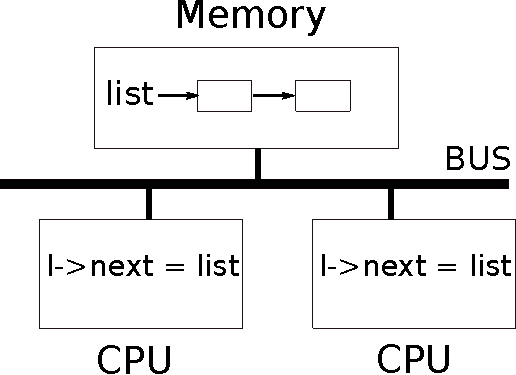
\includegraphics[scale=0.8]{fig/smp.pdf}
\caption{简化的SMP架构  }
\label{fig:smp}
\end{figure}     

作为我们为什么需要锁的一个例子,考虑两个带有退出子进程的进程
 两个不同 CPU 上的  {    \tt    等待   } 。  {    \tt    等待   }  释放子进程的内存。因此每个CPU,内核都会调用 {    \tt    kfree   } 来释放子进程的内存页面。内核分配器维护一个链表:   \lstinline{kalloc()}       \lineref{kernel/kalloc.c:/^kalloc/}    从空闲页列表中弹出一页内存,   \lstinline{kfree()}   
    \lineref{kernel/kalloc.c:/^kfree/}    将页面推送到空闲列表上。为了获得最佳性能,我们可能希望两个父进程的  {    \tt    kfree   }  能够并行执行,而不必等待另一个,但考虑到 xv6 的  {    \tt    kfree   }  实现,这是不正确的。  

图〜   \ref{fig:smp}   更详细地说明了该设置:空闲页面的链接列表位于由两个CPU共享的内存中,这两个CPU使用加载和存储指令来操作该列表。 (实际上,处理器有缓存,但从概念上讲,多处理器系统的行为就好像有一个共享内存一样。)如果没有并发请求,您可以实现列表    \lstinline{push}    操作,如下所示:
    \begin{lstlisting}[numbers=left,firstnumber=1]
    struct element {
      int data;
      struct element *next;
    };
    
    struct element *list = 0;
    
    void
    push(int data)
    {
      struct element *l;
   
      l = malloc(sizeof *l);
      l->data = data;
      l->next = list; (*@\label{line:next}@*)
      list = l;  (*@\label{line:list}@*)
   }
\end{lstlisting}     

   \begin{figure}[t]
\center
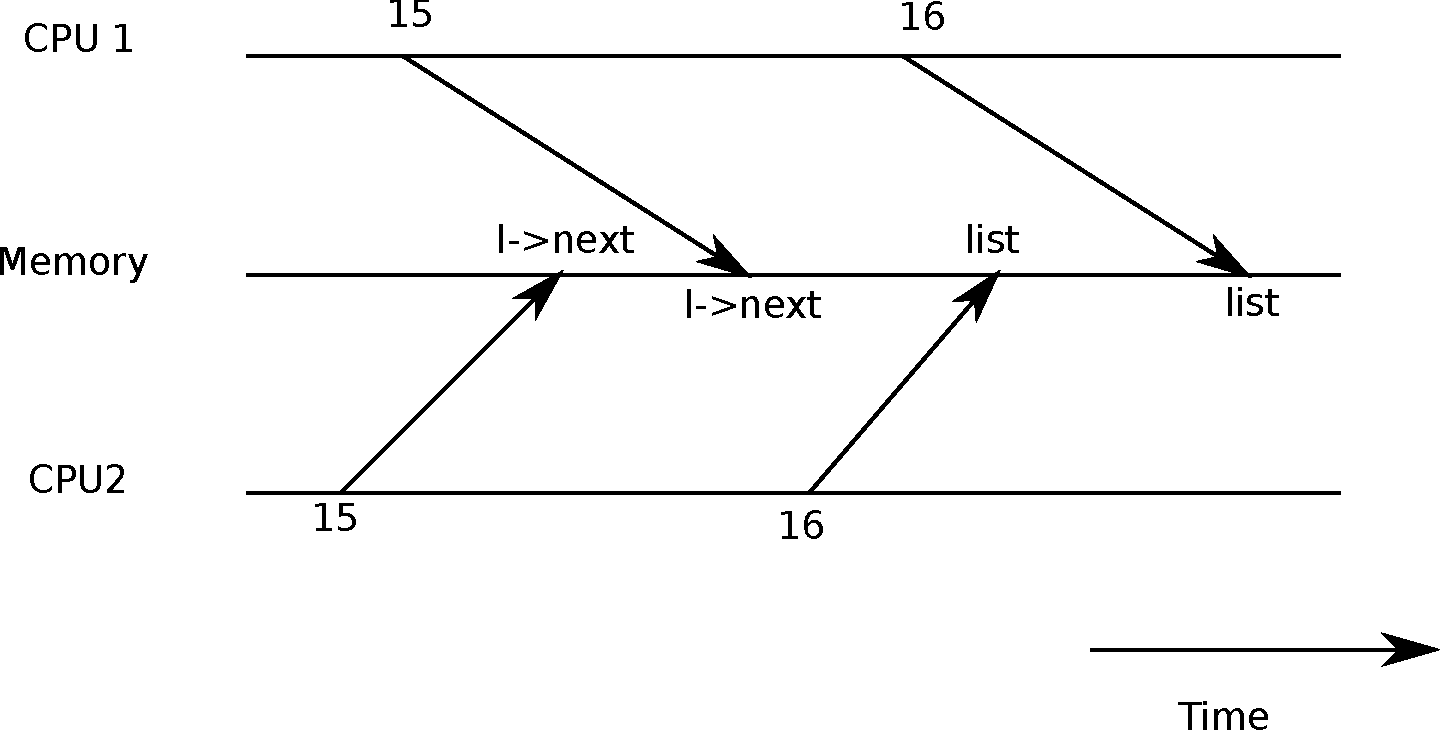
\includegraphics[scale=0.5]{fig/race.pdf}
\caption{比赛示例  }
\label{fig:race}
\end{figure}    如果单独执行,此实现是正确的。但是,如果同时执行多个副本,则代码不正确。如果有两个CPU执行
    \lstinline{push}    同时,两者都可能执行 line~    \ref{line:next}    (如图~    \ref{fig:smp}    所示),然后再执行 line~    \ref{line:list}    ,这会导致错误的结果,如图~    \ref{fig:race}    所示。然后会有twolist元素
    \lstinline{next}    设置为以前的值
    \lstinline{list}   。当两个任务分配到
    \lstinline{list}    发生在 ~    \ref{line:list}    行,第二个将覆盖第一个;第一个赋值涉及的元素将丢失。  

行 ~    \ref{line:list}    处丢失的更新是一个示例
    \indextext{race}    。竞争是一种同时访问内存位置且至少一次访问是写入的情况。竞争通常是错误的迹象,要么是更新丢失(如果访问是写入),要么是读取未完全更新的数据结构。竞争的结果取决于编译器生成的机器代码、所涉及的两个 CPU 的时序以及内存系统如何排序它们的内存操作,这可能会使竞争引起的错误难以重现和调试。例如,调试时添加打印语句
    \lstinline{push}    可能会改变执行的时间,足以使竞争消失。  

避免竞争的常用方法是使用锁。锁确保
    \indextext{mutual exclusion}    ,这样一次只有一个CPU可以执行以下敏感行
    \lstinline{push}    ;这使得上述情况变得不可能。上述代码的正确锁定版本仅添加了几行(以黄色突出显示):
    \begin{lstlisting}[numbers=left,firstnumber=6]
   struct element *list = 0;
   (*@\hl{struct lock listlock;}@*)
    	
   void
   push(int data)
   {
     struct element *l;
     l = malloc(sizeof *l); (*@\label{line:malloc}@*)
     l->data = data;
   
     (*@\hl{acquire( \& listlock);} @*)
     l->next = list;     (*@\label{line:next1}@*)
     list = l;           (*@\label{line:list1}@*)
     (*@\hl{release( \& listlock)}; @*)
   }
\end{lstlisting}    之间的指令序列
    \lstinline{acquire}    和
    \lstinline{release}    通常被称为
    \indextext{critical section}    。锁通常被认为是保护
    \lstinline{list}    。  

当我们说锁保护数据时,我们真正的意思是锁保护一些适用于数据的不变量集合。不变量是跨操作维护的数据结构的属性。通常,操作的正确行为取决于操作开始时不变量是否为真。该操作可能会暂时违反不变量,但必须在完成之前重新建立它们。例如,在链表情况下,不变量是
    \lstinline{list}    指向列表中的第一个元素,并且每个元素的
    \lstinline{next}    字段指向下一个元素。实施
    \lstinline{push}    暂时违反了这个不变量:在~    \ref{line:next1}    行中,
    \lstinline{l}    指向下一个列表元素,但是
    \lstinline{list}    没有指向
    \lstinline{l}    尚未(在 ~    \ref{line:list1}    行重新建立)。我们上面检查的竞争之所以发生,是因为第二个 CPU 执行了依赖于列表不变量的代码,而它们(暂时)被违反了。正确使用锁可以确保一次只有一个 CPU 可以对临界区中的数据结构进行操作,这样当数据结构的不变量不成立时,没有 CPU 会执行该数据结构操作。  

你可以把锁想象成
    \indextext{serializing}    并发关键部分,以便它们一次运行一个,从而保留不变量(假设关键部分单独正确)。您还可以将由同一锁保护的关键部分视为彼此之间的原子性,以便每个关键部分只能看到较早关键部分的完整更改集,而永远不会看到部分完成的更新。  

虽然锁对于正确性很有用,但它本质上限制了性能。例如,如果两个进程同时调用  {    \tt    kfree   } ,锁将序列化两个临界区,因此在不同的 CPU 上运行它们没有任何好处。如果多个进程同时想要相同的锁,则我们说多个进程    \indextext{conflict}    ,或者该锁经历    \indextext{contention}    。内核设计中的一个主要挑战是避免锁争用以追求并行性。 Xv6 几乎没有做到这一点,但复杂的内核专门组织了数据结构和算法来避免锁争用。在列表示例中,内核可以为每个 CPU 维护一个单独的空闲列表,并且仅在当前 CPU 的列表为空并且必须从另一个 CPU 窃取内存时才触及另一个 CPU 的空闲列表。其他用例可能需要更复杂的设计。  

锁的放置对于性能也很重要。例如,移动是正确的
 早些时候的    \lstinline{acquire}   
    \lstinline{push}    ,在行~    \ref{line:malloc}    之前。但这可能会降低性能,因为随后的调用
    \lstinline{malloc}    将被序列化。下面的“使用锁”部分提供了一些关于插入位置的指南
    \lstinline{acquire}    和
    \lstinline{release}    调用。
    \section{代码: 锁  }    Xv6 有两种类型的锁:自旋锁和睡眠锁。我们将从自旋锁开始。 Xv6 将自旋锁表示为
    \indexcode{struct spinlock}   
    \lineref{kernel/spinlock.h:/struct.spinlock/}    。该结构中重要的字段是
    \lstinline{locked}    ,当锁可用时该字为零,而当锁被持有时该字为非零。从逻辑上讲,xv6 应该通过执行类似的代码来获取锁
    \begin{lstlisting}[numbers=left,firstnumber=21]
   void
   acquire(struct spinlock *lk) // does not work!
   {
     for(;;) {
       if(lk->locked == 0) {  (*@\label{line:testlocked}@*)
         lk->locked = 1;      (*@\label{line:assign}@*)
         break;
       }
     }
   }
\end{lstlisting}    不幸的是,此实现不能保证多处理器上的互斥。可能会发生两个 CPU 同时到达线 ~    \ref{line:testlocked}    ,请参阅
    \lstinline{lk->locked}    为零,然后两者都通过执行 line~    \ref{line:assign}    来获取锁。此时,两个不同的CPU持有锁,这违反了互斥性质。我们需要的是一种使    \ref{line:testlocked}    和    \ref{line:assign}    行作为
    \indextext{atomic}   (即不可分割的)步骤。  

由于锁被广泛使用,多核处理器通常提供实现原子版本的指令~    \ref{line:testlocked}    和    \ref{line:assign}    。在 RISC-V 上,这条指令是
    \lstinline{amoswap r, a}    。
    \lstinline{amoswap}    读取内存地址  {    \tt    a   }  处的值,将寄存器  {    \tt    r   }  的内容写入该地址,并将读取到的值放入  {    \tt    r   }  中。也就是说,它交换了寄存器的内容和内存地址。它以原子方式执行此序列,使用特殊硬件来防止任何其他 CPU 使用读取和写入之间的内存地址。  

Xv6的
    \indexcode{acquire}   
    \lineref{kernel/spinlock.c:/^acquire/}    使用可移植 C 库调用
    \lstinline{__sync_lock_test_and_set}    ,归结为
    \lstinline{amoswap}    指令;返回值是旧的(交换的)内容
    \lstinline{lk->locked}    。这
    \lstinline{acquire}    函数将交换包装在循环中,重试(旋转)直到获得锁。每次迭代都会将一个交换为
    \lstinline{lk->locked}    并检查先前的值;如果先前的值为零,那么我们已经获得了锁,并且交换将被设置
    \lstinline{lk->locked}    比 1。如果前一个值是 1,则其他某个 CPU 持有该锁,并且我们以原子方式将 1 交换为
    \lstinline{lk->locked}    没有改变它的值。  

一旦获得锁,
    \lstinline{acquire}    记录获取锁的 CPU,以供调试。这
    \lstinline{lk->cpu}    字段受锁保护,并且只能在持有锁时更改。  

功能
    \indexcode{release}   
    \lineref{kernel/spinlock.c:/^release/}    与
    \lstinline{acquire}    :它清除
    \lstinline{lk->cpu}    字段,然后释放锁。从概念上讲,该版本只需要将零分配给
    \lstinline{lk->locked}    。 C 标准允许编译器使用多个存储指令实现赋值,因此 C 赋值对于并发代码来说可能是非原子的。反而,
    \lstinline{release}   使用C库函数
 执行原子赋值的    \lstinline{__sync_lock_release}   。该功能也归结为 RISC-V
    \lstinline{amoswap}    指令。
    \section{代码:使用锁  }    Xv6 在许多地方使用锁来避免竞争。如上所述,
    \lstinline{kalloc}   
    \lineref{kernel/kalloc.c:/^kalloc/}    和
    \lstinline{kfree}   
    \lineref{kernel/kalloc.c:/^kfree/}    就是一个很好的例子。尝试练习 1 和 2,看看如果这些函数忽略锁会发生什么。您可能会发现很难触发不正确的行为,这表明很难可靠地测试代码是否没有锁定错误和竞争。 Xv6 很可能有尚未被发现的种族。  

使用锁的一个困难部分是决定使用多少个锁以及每个锁应保护哪些数据和不变量。有一些基本原则。首先,只要一个 CPU 可以写入变量,同时另一个 CPU 可以读取或写入该变量,则应使用锁来防止两个操作重叠。其次,请记住锁保护不变量:如果不变量涉及多个内存位置,通常所有这些位置都需要由单个锁保护以确保不变量得到维护。  

上面的规则说明了何时需要锁,但没有提及何时不需要锁,并且不要锁太多对于效率很重要,因为锁会降低并行性。如果并行性不重要,那么可以安排只有一个线程而不用担心锁。简单的内核可以在多处理器上通过拥有一个锁来做到这一点,该锁必须在进入内核时获取并在退出内核时释放(尽管会阻塞系统调用,例如管道读取或
    \lstinline{wait}    会造成问题)。许多单处理器操作系统已使用这种方法转换为在多处理器上运行,有时称为“大内核锁”,但该方法牺牲了并行性:一次只有一个 CPU 可以在内核中执行。如果内核执行任何繁重的计算,那么使用更大的一组更细粒度的锁会更有效,以便内核可以同时在多个CPU上执行。  

作为粗粒度锁定的示例,xv6 的    \lstinline{kalloc.c}    分配器具有受单个锁保护的单个空闲列表。如果不同 CPU 上的多个进程尝试同时分配页面,则每个进程都必须通过在  {    \tt    获取   }  中旋转来等待轮到它。旋转会浪费 CPU 时间,因为它不是有用的工作。如果锁争用浪费了很大一部分 CPU 时间,也许可以通过更改分配器设计来提高性能,使其具有多个空闲列表,每个列表都有自己的锁,以允许真正的并行分配。  

作为细粒度锁定的一个示例,xv6 对每个文件都有一个单独的锁,因此操作不同文件的进程通常可以继续执行而无需等待彼此的锁。如果希望允许进程同时写入同一文件的不同区域,则可以使文件锁定方案变得更加细粒度。最终,锁粒度决策需要由性能测量和复杂性考虑来驱动。  

后续章节在解释 xv6 的各个部分时,会提到 xv6 使用锁来处理并发的示例。作为预览,图~    \ref{fig:locktable}    列出了 xv6 中的所有锁。  

   \begin{figure}[t]
\center
\begin{tabular}{ll}
{\bf Lock} & {\bf Description}  \\ 
\midrulebcache.lock & Protects allocation of block buffer cache entries  \\ cons.lock & Serializes access to console hardware, avoids intermixed output  \\ ftable.lock & Serializes allocation of a struct file in file table  \\ itable.lock & Protects allocation of in-memory inode entries  \\ vdisk\_lock & Serializes access to disk hardware and queue of DMA descriptors  \\ kmem.lock & Serializes allocation of memory  \\ log.lock & Serializes operations on the transaction log  \\ pipe's pi->lock & Serializes operations on each pipe  \\ pid\_lock & Serializes increments of next\_pid  \\ proc's p->lock & Serializes changes to process's state  \\ wait\_lock & Helps wait avoid lost wakeups  \\ tickslock & Serializes operations on the ticks counter  \\ inode's ip->lock & Serializes operations on each inode and its content  \\ buf's b->lock & Serializes operations on each block buffer  \\ 
\end{tabular}
\caption{锁定 xv6  }
\label{fig:locktable}
\end{figure}   
    \section{死锁和锁顺序  }    如果通过内核的代码路径必须同时持有多个锁,则所有代码路径以相同的顺序获取这些锁非常重要。如果不这样做,则存在    \indextext{deadlock}    的风险。假设有两条代码路径 inxv6 需要锁 A 和 B,但是代码路径 1 按照 Athen B 的顺序获取锁,而另一条路径则按照 B 然后 A 的顺序获取锁。假设线程 T1 执行代码路径 1 并获取锁 A,并且线程 T2 执行代码路径 2 并获取锁 B。接下来,T1 将尝试获取锁 B,T2 将尝试获取锁 A。这两种获取都会无限期地阻塞,因为在这两种情况下,另一个线程都持有所需的锁,并且不会释放它直到它获取返回。为了避免此类死锁,所有代码路径必须以相同的顺序获取锁。对全局锁获取顺序的需求意味着锁实际上是每个函数规范的一部分:调用者必须以导致按照商定的顺序获取锁的方式调用函数。  

Xv6 有许多长度为 2 的锁顺序链,涉及每个进程锁(每个进程中的锁)
    \lstinline{struct proc}    )由于这样的方式
    \lstinline{sleep}    有效(参见章节~    \ref{CH:SCHED}    )。例如,
    \lstinline{consoleintr}   
    \lineref{kernel/console.c:/^consoleintr/}    是处理键入字符的中断例程。当换行符到达时,任何正在等待控制台输入的进程都应该被唤醒。去做这个,
    \lstinline{consoleintr}    成立
 通话时    \lstinline{cons.lock}   
    \indexcode{wakeup}    ,它获取等待进程的锁以唤醒它。因此,全局死锁避免锁顺序包括以下规则:
 必须在任何进程锁之前获取    \lstinline{cons.lock}   。文件系统代码包含 xv6 最长的锁链。例如,创建文件需要同时持有目录上的锁、新文件的 inode 上的锁、磁盘块缓冲区上的锁、磁盘驱动程序的    \lstinline{vdisk_lock}    和调用进程的    \lstinline{p->lock}    。为了避免死锁,文件系统代码始终按照上一句中提到的顺序获取锁。  

遵守全球避免僵局的秩序可能异常困难。有时,锁定顺序与逻辑程序结构冲突,例如,代码模块 M1 可能调用模块 M2,但锁定顺序要求先获取 M2 中的锁,然后再获取 M1 中的锁。有时,锁的身份事先并不知道,也许是因为必须持有一个锁才能发现下一个要获取的锁的身份。这种情况出现在文件系统中,因为它在路径名中查找连续的组件,并且在  {    \tt    等待   }  和  {    \tt    退出   }  的代码中,当它们搜索进程表以查找子进程时。最后,死锁的危险通常是对锁定方案的细粒度程度的限制,因为更多的锁通常意味着更多的死锁机会。避免死锁的需要通常是内核实现的一个主要因素。  

   \section{可重入锁  }     

使用    \indextext{re-entrant locks}   (也称为    \indextext{recursive locks}   )似乎可以避免一些死锁和锁排序挑战。这个想法是,如果锁被一个进程持有,并且该进程尝试再次获取锁,那么内核可以允许这样做(因为该进程已经拥有锁),而不是像 xv6 内核那样调用恐慌。  

然而,事实证明,可重入锁使推理并发性变得更加困难:可重入锁打破了锁导致临界区相对于其他临界区是原子的直觉。考虑以下两个函数    \lstinline{f}    和
    \lstinline{g}   :  

   \begin{lstlisting}struct spinlock lock;int data = 0; // protected by lock

f() {
  acquire(&lock);
  if(data == 0){
    call_once();
    h();
    data = 1;
  }
  release(&lock);
}

g() {
  aquire(&lock);
  if(data == 0){
    call_once();
    data = 1;
  }
  release(&lock);
}
\end{lstlisting}     

看看这个代码片段,直觉是
    \lstinline{call_once}    将仅被调用一次:由    \lstinline{f}    或    \lstinline{g}    调用,但不能同时由两者调用。  

但是如果允许重入锁,并且    \lstinline{h}    恰好调用
    \lstinline{g}   、   \lstinline{call_once}   将被调用两次。  

如果不允许重入锁,则    \lstinline{h}    调用
    \lstinline{g}    会导致死锁,这也不是很好。但是,假设调用将是一个严重的错误
    \lstinline{call_once}    ,最好是死锁。内核开发人员将观察死锁(内核恐慌),并可以修复代码以避免死锁,同时调用
    \lstinline{call_once}    两次可能会默默地导致难以追踪的错误。  

为此,xv6 使用了更容易理解的不可重入锁。然而,只要程序员牢记锁定规则,任何一种方法都可以发挥作用。如果 xv6 要使用重入锁,则必须修改    \lstinline{acquire}    才能注意到该锁当前由调用线程持有。还必须向 struct spinlock 添加嵌套获取的计数,其风格与    \lstinline{push_off}    类似,这将在接下来讨论。  

   \section{锁和中断处理程序  }   
    \label{s:lockinter}    一些 xv6 自旋锁保护线程和中断处理程序使用的数据。例如,
    \lstinline{clockintr}    定时器中断处理程序可能会增加
    \indexcode{ticks}   
    \lineref{kernel/trap.c:/^clockintr/}    大约在内核线程读取的同时
    \lstinline{ticks}    中
    \indexcode{sys_sleep}   
    \lineref{kernel/sysproc.c:/ticks0.=.ticks/}   。锁
    \indexcode{tickslock}    序列化这两个访问。  

自旋锁和中断的相互作用会带来潜在的危险。认为
    \indexcode{sys_sleep}    成立
    \indexcode{tickslock}   ,其CPU被定时器中断中断。
    \lstinline{clockintr}    会尝试获取
    \lstinline{tickslock}    ,看到它被持有,并等待它被释放。在这个情况下,
    \lstinline{tickslock}    永远不会发布:仅
    \lstinline{sys_sleep}   可以释放它,但是
    \lstinline{sys_sleep}    将不会继续运行,直到
    \lstinline{clockintr}    返回。因此,CPU 将发生死锁,并且任何需要任一锁的代码也将冻结。  

为了避免这种情况,如果中断处理程序使用自旋锁,则 CPU 绝不能在启用中断的情况下持有该锁。 Xv6 更加保守:当 CPU 获取任意锁时,xv6 始终禁用该 CPU 上的中断。中断可能仍会发生在其他 CPU 上,因此中断的
    \lstinline{acquire}   可以等待线程释放自旋锁;只是不在同一个CPU上。  

当 CPU 没有自旋锁时,Xv6 重新启用中断;它必须做一些簿记来处理嵌套的关键部分。
    \lstinline{acquire}    次调用
    \indexcode{push_off}   
    \lineref{kernel/spinlock.c:/^push_off/}    和
    \lstinline{release}    调用
    \indexcode{pop_off}   
    \lineref{kernel/spinlock.c:/^pop_off/}    跟踪当前 CPU 上锁的嵌套级别。当该计数达到零时,
    \lstinline{pop_off}    恢复最外层临界区开始处存在的中断使能状态。这
    \lstinline{intr_off}    和
    \lstinline{intr_on}    函数执行 RISC-V 指令来分别禁用和启用中断。  

重要的是
    \indexcode{acquire}    调用
    \lstinline{push_off}    严格在设置之前
    \lstinline{lk->locked}   
    \lineref{kernel/spinlock.c:/sync_lock_test_and_set/}    。如果两者颠倒,则在启用中断的情况下保持锁定时会出现一个短暂的窗口,不幸的是定时中断将使系统死锁。同样,重要的是
    \indexcode{release}    调用
    \indexcode{pop_off}    仅在释放锁后
    \lineref{kernel/spinlock.c:/sync_lock_release/}    。
    \section{指令和内存排序  }     

人们很自然地认为程序是按照源代码语句出现的顺序执行的。对于单线程代码来说,这是一个合理的心理模型,但当多个线程通过共享内存交互时,这是不正确的~    \cite{riscv:user,boehm04}    。原因之一是编译器发出加载和存储指令的顺序与源代码所暗示的顺序不同,并且可能完全省略它们(例如通过在寄存器中缓存数据)。另一个原因是CPU可能会乱序执行指令以提高性能。例如,CPU 可能会注意到指令 A 和 B 的串行序列中并不相互依赖。 CPU 可能会首先启动指令 B,要么是因为其输入在 A 的输入之前准备好,要么是为了重叠执行 A 和 B。  

作为可能出错的示例,在这段代码中
    \lstinline{push}    ,如果编译器或 CPU 将对应于 line~    \ref{line:next2}    的存储移动到该行之后的点,那将是一场灾难
    \lstinline{release}   上线~    \ref{line:release}   :
    \begin{lstlisting}[numbers=left,firstnumber=1]
      l = malloc(sizeof *l);
      l->data = data;
      acquire(&listlock);
      l->next = list;   (*@\label{line:next2}@*)
      list = l;      
      release(&listlock);  (*@\label{line:release}@*)
\end{lstlisting}    如果发生这样的重新排序,将会出现一个窗口,在此期间另一个 CPU 可以获取锁并观察更新的结果
    \lstinline{list}    ,但看到一个未初始化的
    \lstinline{list->next}    。  

好消息是,编译器和 CPU 遵循一组称为    \indextext{memory model}    的规则,并提供一些原语来帮助程序员控制重新排序,从而帮助并发程序员。  

为了告诉硬件和编译器不要重新排序,xv6 使用
 两者均    \lstinline{__sync_synchronize()}   
    \lstinline{acquire}       \lineref{kernel/spinlock.c:/^acquire/}    和
    \lstinline{release}       \lineref{kernel/spinlock.c:/^release/}    。
    \lstinline{__sync_synchronize()}    是    \indextext{memory barrier}    :它告诉编译器和 CPU 不要跨障碍重新排序加载或存储。 xv6 中的障碍
    \lstinline{acquire}    和
    \lstinline{release}    在几乎所有重要的情况下都强制执行顺序,因为 xv6 在共享数据的访问周围使用锁。第~    \ref{CH:LOCK2}    章讨论了一些例外情况。
    \section{睡眠锁  }     

有时xv6需要长时间持有锁。例如,文件系统(Chapter~    \ref{CH:FS}   )在磁盘上读取和写入文件内容时保持文件锁定,这些磁盘操作可能需要数十毫秒。如果另一个进程想要获取自旋锁,那么长时间持有该自旋锁会导致浪费,因为获取进程会在自旋时长时间浪费 CPU。自旋锁的另一个缺点是进程在保留自旋锁的同时无法让出 CPU。我们希望这样做,以便其他进程可以在拥有锁的进程等待磁盘时使用 CPU。持有自旋锁时让出是非法的,因为如果第二个线程随后尝试获取自旋锁,可能会导致死锁;由于  {    \tt    获取   }  不让出 CPU,第二个线程的自旋可能会阻止第一个线程运行并释放锁。在持有锁时让出也会违反在持有自旋锁时中断必须关闭的要求。因此,我们需要一种在等待获取时让出 CPU,并在持有锁时允许让出(和中断)的锁。  

Xv6 以以下形式提供此类锁
    \indextext{sleep-locks}    。
    \lstinline{acquiresleep}   
    \lineref{kernel/sleeplock.c:/^acquiresleep/}    在等待时使用 CPU,使用的技术将在第    \ref{CH:SCHED}    章中解释。在较高级别上,睡眠锁具有
 由自旋锁保护的    \lstinline{locked}    字段,以及
    \lstinline{acquiresleep}    '调用
    \lstinline{sleep}    以原子方式让出 CPU 并释放自旋锁。结果是其他线程可以执行 while
    \lstinline{acquiresleep}    等待。  

由于睡眠锁使中断保持启用状态,因此它们不能在中断处理程序中使用。因为
    \lstinline{acquiresleep}    可能会占用 CPU,睡眠锁不能在自旋锁关键部分内使用(尽管自旋锁可以在睡眠锁关键部分内使用)。  

自旋锁最适合短临界区,因为等待它们会浪费 CPU 时间;睡眠锁非常适合长时间操作。
    \section{真实世界  }    尽管对并发原语和并行性进行了多年的研究,但使用锁进行编程仍然具有挑战性。通常最好在同步队列等更高级别的构造中隐藏锁,尽管 xv6 没有这样做。如果您使用锁进行编程,那么明智的做法是使用尝试识别竞争的工具,因为很容易错过需要锁的不变量。  

大多数操作系统支持 POSIX 线程 (Pthreads),它允许用户进程在不同的 CPU 上同时运行多个线程。 Pthreads 支持用户级锁、屏障等。Pthreads 还允许程序员有选择地指定锁应该是可重入的。  

在用户级别支持 Pthreads 需要操作系统的支持。例如,如果一个 pthread 在系统调用中阻塞,则同一进程的另一个 pthread 应该能够在该 CPU 上运行。作为另一个示例,如果 pthread 更改其进程的地址空间(例如,映射或取消映射内存),则内核必须安排运行同一进程的线程的其他 CPU 更新其硬件页表以反映地址空间中的更改。  

可以在没有原子指令的情况下实现锁~    \cite{lamport:bakery}    ,但它很昂贵,并且大多数操作系统都使用原子指令。  

如果许多 CPU 尝试同时获取相同的锁,那么锁的成本可能会很高。如果一个 CPU 在其本地缓存中缓存了一个锁,而另一个 CPU 必须获取该锁,则更新持有该锁的缓存行的原子指令必须将该行从一个 CPU 的缓存移动到另一个 CPU 的缓存,并且可能会使任何其他副本无效缓存行的。从另一个 CPU 的高速缓存中获取高速缓存行的成本可能比从本地高速缓存中获取高速缓存行的成本高出几个数量级。  

为了避免与锁相关的开销,许多操作系统使用无锁数据结构和算法~    \cite{herlihy:art,mckenney:rcuusage}    。例如,可以实现像本章开头那样的链表,在列表搜索期间不需要锁,并且需要一条原子指令在列表中插入一项。然而,无锁编程比锁编程更复杂。例如,我们必须担心指令和内存的重新排序。使用锁编程已经很困难,因此 xv6 避免了无锁编程的额外复杂性。
    \section{练习  }     

   \begin{enumerate}

 
   \item   注释掉以下调用
    \lstinline{acquire}    和
    \lstinline{release}    中
    \lstinline{kalloc}   
    \lineref{kernel/kalloc.c:/^kalloc/}    。这似乎应该会导致调用的内核代码出现问题
    \lstinline{kalloc}    ;您预计会看到什么症状?当您运行 xv6 时,您是否看到这些症状?跑步的时候怎么样
    \lstinline{usertests}   ?如果您没有发现问题,为什么不呢?看看是否可以通过将虚拟循环插入到关键部分来引发问题
    \lstinline{kalloc}    。   \item   假设您注释掉了锁定
    \lstinline{kfree}   (恢复锁定后
    \lstinline{kalloc}   )。现在可能会出现什么问题?是否缺少锁
    \lstinline{kfree}    的危害性比
    \lstinline{kalloc}   ?   \item   如果两个CPU调用
    \lstinline{kalloc}    同时,一个必须等待另一个,这对性能不利。调整
    \lstinline{kalloc.c}    具有更多并行性,以便同时调用
 来自不同CPU的   \lstinline{kalloc}   可以继续进行而无需互相等待。   \item   使用大多数操作系统都支持的 POSIX 线程编写并行程序。例如,实现一个并行哈希表并测量放入/获取的数量是否随着核心数量的增加而变化。   \item   在 xv6 中实现 Pthread 的子集。即实现一个用户级线程库,使得一个用户进程可以有1个以上的线程,并安排这些线程可以在不同的CPU上并行运行。提出一种设计,可以正确处理线程进行阻塞系统调用并更改其共享地址空间。  \end{enumerate}     

\end{document}

